\documentclass{report}

\usepackage{graphicx}
\usepackage{palatino} % lettertype
\usepackage{hyperref}
\usepackage{eurosym}
\usepackage{tikz}
\usetikzlibrary{arrows}

\newcommand{\mychapter}[2]{
    \setcounter{chapter}{#1}
    \setcounter{section}{0}
    \chapter*{#2}
    \addcontentsline{toc}{chapter}{#2}
}
\frenchspacing

%In case of edits, please add authors by \and and do not remove older ones
\title{Script Treasurer}
\author{Tjeerd Jan Heeringa\\
	\texttt{+316 3442 6776}	
}
\date{\today}

\begin{document}
\maketitle
\section*{Preamble}
This is the script for the current or upcoming treasurer of Abacus. This document has been written to reduce the risk of loss of knowledge from treasurer to treasurer. It has been written as been spoken or addressed to the treasurer only. Nonetheless if you, the reader, are not the current or upcoming treasurer of Abacus, this script will be able to teach you how the bookkeeping within Abacus works and what the main ideas are behind every aspect of the [ambacht]. The content has been broken down in 3 chapters. The first is focusing on the analog aspects of being the treasurer like the daily tasks. The second chapter is about the digital part, which contains for example the programs you use and the way the journal are grouped. The third and last chapter is the appendix. In the appendix all residual information has been put, just as an easy overview of what each term used in the document means.       

\tableofcontents

\mychapter{1}{Tasks of the Treasurer}
In your duty as a treasurer it is your task to ensure all money flows are flowing properly. This chapter will cover your main tasks and give a appropriate explanation of what those mean. Subsidiary explanations can be found in the addendum. Your main tasks are the following:
\begin{itemize} 
\vspace{-1mm}
\itemsep-1mm
\item Make financial reports
\item Instruct and guide the committee treasurers
\item Maintain and document the money flows
\item Buy and sell products for Abacus
\end{itemize}


\section{Make financial reports}
Every year in a treasurers live starts with a plan of what he or she is going to spend and ends his or her year with a report on what has been spend during the year. Within Abacus we also include a report halfway through the year with a renewed plan for the second half year based on the results of the first half of the year. with Abacus the year starts on the first of August and ends at the thirty-first of July the year after. This implies that the year is halfway on the first of February. \\
Next to these major financial reports you also have to make some minor financial reports for the activities organized by the board. For a specification on how to make all these financial reports read on below. For explanation of what should be put on what post, please look in the addendum.   

\subsection{Budget}

\begin{itemize} 
\vspace{-1mm}
\itemsep-1mm 
\item 
\end{itemize}

\subsection{Half year financial report}

\begin{itemize} 
\vspace{-1mm}
\itemsep-1mm 
\item 
\end{itemize}

\subsection{Whole year financial report}

\begin{itemize} 
\vspace{-1mm}
\itemsep-1mm 
\item 
\end{itemize}

\subsection{Minor financial reports}
auditing committee
financial update
\begin{itemize} 
\vspace{-1mm}
\itemsep-1mm 
\item 
\end{itemize}

\section{Instruct and guide the committee treasurers}

\subsection{Give instruction to how to be a treasurer}
\begin{itemize} 
\vspace{-1mm}
\itemsep-1mm 
\item 
\end{itemize}

\subsection{Review budget}
\begin{itemize}
\vspace{-1mm}
\itemsep-1mm 
\item
\end{itemize}

\subsection{Review financial report}
\begin{itemize} 
\vspace{-1mm}
\itemsep-1mm 
\item 
\end{itemize}

\section{Maintain the money flows}
After you and your board have established the plans for the year to come, these plans have to be realized. This realization of plans flows from proper management of the monetary flows within the association. Each of these flows will be [behandeld] in the following chapters. Everything about these flows will have to be stored digital and on paper for the sake of security. The reason for this can be found in the appendix\ref{A}. The paper journals have to placed in ledger having proper and descriptive names on their backs.   

\subsection{Creditor}
The first flow that comes to mind is possibly the outgoing flow. The treasurer is the person who pays the stuff for the association. The treasurer pays according to payment requests, which can be broadly categorized into two groups: invoices and declarations. Characteristics of these groups are that they have separate forms and the person filling in the form tends to be no member respectively a member of the association. Each specific person that submits a valid requests is called a creditor(think of owing someone some credit), hence the name for the category. For both groups some similarities in the way you need to treat them is present. Most importantly you need to check whether the information present is valid information. Secondly the request has to be handled within the time given for it.          

\subsubsection{Invoice}
Invoices are the payment requests forms usually used by companies. These can come in many different formats and styles, but all share some common information. See in the appendix for the exact information needed to be mentioned on a invoice to be valid\ref{A}. Mentioned above is that the primary task is to check whether an invoice is valid. In the appendix you can see that there are a whole lot of requirements to be met for it to be valid. Some information can be used to really see quickly if it is valid or not and some information is nearly impossible or simply impractical to check. Basically you or obliqued to check the following:
\begin{itemize} 
	\vspace{-1mm}
	\itemsep-1mm 
	\item The origin of the invoice
	\item The service or good wherefore the invoice is sent
	\item The amount
	\item Bank account*
\end{itemize}
The other information is for the companies to present correctly as this has to be shown to the government and erroneous data outside the above mentioned is of no consequence for the association. The above can be verified by the following methods in order of introduction:
\begin{itemize} 
	\vspace{-1mm}
	\itemsep-1mm 
	\item The invoice came from the person that was also the person with whom the deal for the services or goods was made
	\item The deal closed or contract signed for which this invoice is sent has to have the same services and goods as is on the invoice
	\item The deal closed or contract signed has a price and this should be the same as the invoice
	\item Every time you do a transaction the bank account is saved, therefore this can only be checked by invoices of earlier creditors. This bank account number you used last time should be the same as the current number if no other notices of the creditor about this are given  
\end{itemize} 
In case of mistakes or uncertainties you should contact the sender of the invoice or the person with whom the deal was closed or the contract was signed to resolve this issues. When the invoice is deemed valid by you, it is time to book it. How to digital book it, can be found in the appendix\ref{A}. The digital booking gives you a number that relates the paper invoice to the digital entry, usually being the number of the last invoice added to the journals incremented by one. This number should be placed on the top of the invoice. After writing the number, the invoice should be added to the corresponding ledger. The last thing that remains is to pay the invoice in due time. This is best to be done digitally. After paying the invoice should be stamped with the payment date.

\subsubsection{Declaration}
The second type of payment request is the declaration. This is usually filed by members of the association and is in a format chosen by the treasurer. The exact requirements for the form can be found in the appendix\ref{A}. This type of document is most likely the type you will be seeing most often during your year as treasurer. To check a declaration you should see if all mentioned fields are filled in correctly. If this is the case then you can go ahead and declare it valid, yet if this is not the case the declaration should be corrected. The correction can either be done by the person who filed it or the treasurer. The board represented by you is all cases able to declare a declaration valid although not all information has been submitted properly. To declare a declaration valid your signature is required in the field reserved for it. After deeming a declaration valid you have to enter it digitally\ref{A}. This digital booking gives you a reference number to relate the declaration to the digital entry, usually being the number of the last declaration added to the journals incremented by one. This number should be placed in the designated field. Place the declaration in de corresponding ledger. When the declaration gets paid, the declaration needs to get a stamp with the payment date in the designated field.        

\subsection{Debtor}
Just as you are able to receive request for payments, so are you also able to sent them to others. The persons you sent a request for payment to are called debtors, since they have some kind of debt to you. These requests for payment you send, typically are either invoices or notices for an direct debit. Invoices and direct debits have different requirements for them to be valid. The following paragraphs will explain how you should threat them. 

\subsubsection{Invoice}
Once in a while someone buys stuff from Abacus, gets a service provided for by Abacus or sponsors Abacus. To get the money from that party a request for payment has to be done. This is done in the form of an invoice. Invoices are almost always the same in layout from one to the other. What requirements these invoices have can be found in the appendix\ref{A}. Contrary to the invoices you receive, you need to make sure that each and every field is correct. How to make and send the invoices can be found in chapter 2 Multiverse under the debtor section\ref{A}. After sending the invoice, the invoice has to archived in the proper ledger with the digital reference number written on the top side.    

\subsubsection{Direct debit}
All lot of the payments within Abacus are linked to people their accounts. A benefit by having such a system is that not for every payment an invoice has to be send. Direct debit are a possibility given by this system. As soon as the people have given you permission to use their accounts, you can sent them a direct debit for the costs they have made. This can given for all of the costs made by the person. Within Abacus this means that permission can be given for all of the following: 
\begin{itemize} 
	\vspace{-1mm}
	\itemsep-1mm 
	\item Activities
	\item Contribution
	\item Cookie Terminal
	\item Drinks
\end{itemize}
For those that do not give you permission for a direct debit, you have to make invoices for all payments you require from them. As these direct debits are a gathering of a lot of payments, the usage of them greatly reduces the amount of work you have to do. How to make and sent the direct debits can be found in chapter 2 Multiverse\ref{A}. More information on the specific types and requirements can be found in the appendix\ref{A}.  

\subsection{Cash}
In the above subsections we have seen the outgoing flow and the incoming flow of money. The thing that remains is what cannot be placed in either of the two flows. Careful ready of the both reveals that the two flows cover all transactions with a person or company whereby the person or company is known by an account, closed deal or signed contract. This leaves the transactions were the persons is known or recorded. In Abacus this is only with the cash transactions. Note that this does not apply to all cash transaction as for some things cash payments is required. Not knowing or tracking the person is however no reason to leave these transactions unmanaged. Individual transaction cannot be monitored, but the bulk can be. The way this is done is by preparing a money box for each activity or drink for which is known or expected that there might be cash transactions done. By recording the initial value and the final value of the content of the money box, the sum of the cash transactions can be determined. The final amount will be split into an amount equal to the initial value and the difference between the initial and final value. The difference is equal to the sum of the cash transactions performed. To record all these values there is a case book. The case book gets an entry for every cash transaction with the person or company known or tracked and gets an entry for the initial value of the money box at the time the money is taken from the safe and an entry for both the initial value and the difference at the time the money is taken from the money box and put back into the safe. All these values should be ordered chronologically. For how to record this digitally, read the sections in chapter 2 Multiverse\ref{A}. More information for the requirements on a cash book can be found in the appendix\ref{A}.   

\section{Buy and sell products for Abacus}

\subsection{Food}

\subsubsection{Procurement}
\begin{itemize} 
\vspace{-1mm}
\itemsep-1mm 
\item 
\end{itemize}

\subsubsection{Sale}
\begin{itemize}
\vspace{-1mm}
\itemsep-1mm 
\item
\end{itemize}

\subsection{Drinks}
\subsubsection{Procurement}
Abacus is part of the association SBZ, Stichting Borrelbeheer Zilverling. All drinks we buy are bought there. At the end of every drink the administrating system for drink called alex.ia will be updated by the barkeepers. For every month you will get an invoice. This invoice will contain all drinks bought with their respective amount. Once you get such an invoice, pay attention to the following:  
\begin{itemize} 
\vspace{-1mm}
\itemsep-1mm 
\item Is the drink a drink that Abacus organized
\item Which committee organized the drink
\item Is the amount we bought reasonable
\item Did we give drinks for free or were there any special sales
\end{itemize}
In the case that Abacus did not organize the drink or the amounts on the invoice are off, make contact with the treasurer of SBZ to opt for a correction invoice.

Once you validated the invoice, it has to be separated in a part for external drinks and ordinary drinks. All posts of the invoice have to spread out over these two posts with the same content in them. If some drinks were given for free or some special offers were made, the costs for those should not be placed on the mentioned posts above but on the organizing committee.  

\subsubsection{Sale}
During drinks payment is done either in cash or by tap. All cash payments will go to the safe provided to the barkeepers. More reading on this can be found in CASH. Paying drinks on tap is done by alex.ia, de administration system for drinks. All drinks are registered through alex.ia on the abacuswebsite.  

\subsection{Stock}
\subsubsection{Procurement}
\begin{itemize} 
\vspace{-1mm}
\itemsep-1mm 
\item 
\end{itemize}

\subsubsection{Sale}
\begin{itemize}
\vspace{-1mm}
\itemsep-1mm 
\item
\end{itemize}




\newpage
\mychapter{2}{Multivers}
Multivers is the accounting program you will be using. It serves as the digital collection of all your financial actions and transactions. The use of such a program greatly enhances the overview you have and greatly reduces the amount of errors going unnoticed. In the following subsections you will be explained how to use the program.
\section{Creditors, Debtors and Declarations}
\section{Waste-book/Memorial}
\section{Ledger/Cash book}
\section{Bankbook}
\section{Balance sheet}
\section{Back-up}
As for any digital system it is necessary to make regular back-ups to ensure that in case of a crash a minimal amount of data is lost or has to be entered again. You can make a back-up by doing the following:
\begin{itemize}
	\item 
	\item 
	\item 
\end{itemize} 

\section{Images}
\begin{figure}
	\centering
	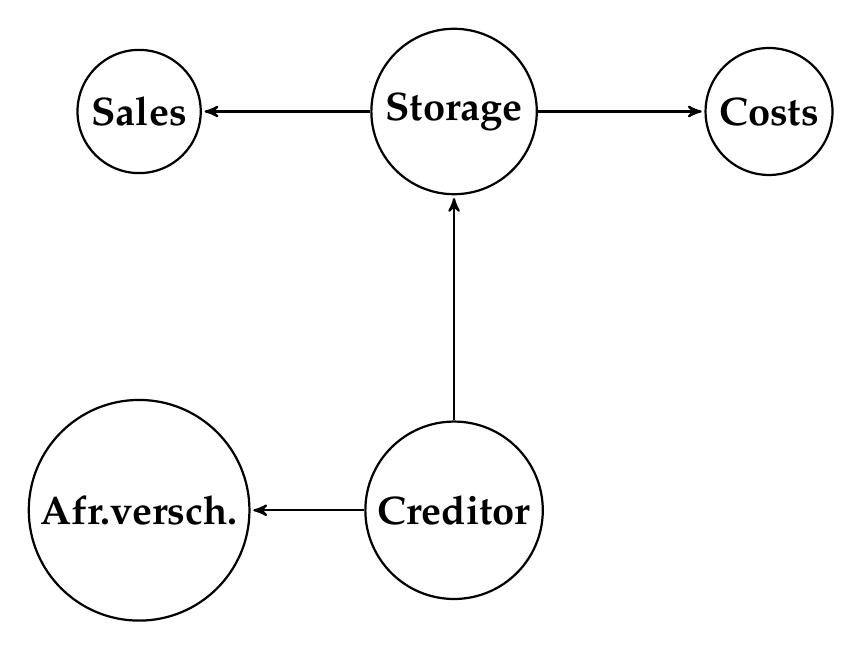
\begin{tikzpicture}[->,>=stealth',shorten >=1pt,auto,node distance=4cm,
	thick,main node/.style={circle,draw,font=\Large\bfseries}]
	
	\node[main node] (a) [midway]{Storage};
	\node[main node] (d) [midway, below of=a] {Creditor};
	\node[main node] (b) [left of=d] {Afr.versch.};
	\node[main node] (c) [right of=a] {Costs};
	\node[main node] (e) [left of=a] {Sales};
	
	\path
	(d) edge node {} (a)
	(d) edge node {} (b)
	(a) edge node {} (c)
	(a) edge node {} (e);
	\end{tikzpicture}
	\caption{Flow chart for Stock}
\end{figure}
\begin{figure}
	\centering
	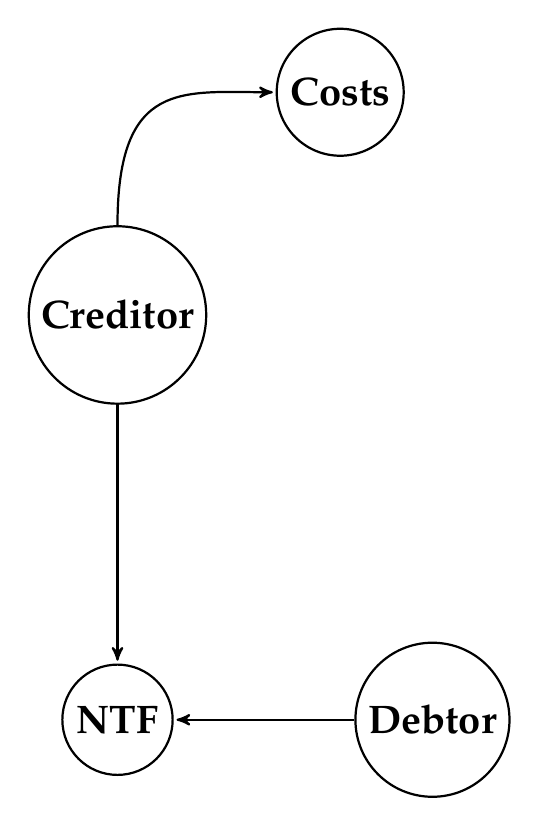
\begin{tikzpicture}[->,>=stealth',shorten >=1pt,auto,node distance=4cm,
	thick,main node/.style={circle,draw,font=\Large\bfseries}]
	
	\node[main node] (a) [midway]{Creditor};
	\node[main node] (d) [midway, below of=a] {NTF};
	\node[main node] (c) [above right of=a, align=right] {Costs};
	\node[main node] (e) [right of=d] {Debtor};
	
	\path
	(a) edge node {} (d)
	(e) edge node {} (d);
	\draw [->] (a) .. controls +(up:3cm) and +(left:2cm) .. node[above,sloped] {} (c);
	\end{tikzpicture}
	\caption{Flow chart for SBZ invoices}
\end{figure}
\begin{figure}
	\centering
	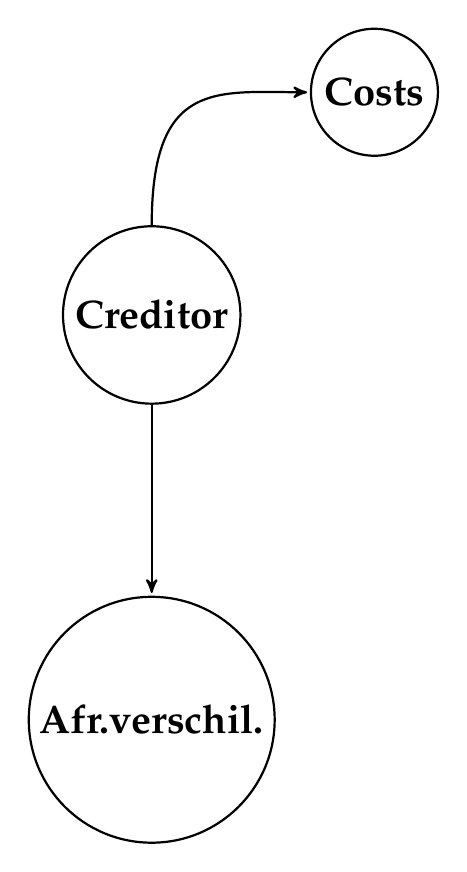
\begin{tikzpicture}[->,>=stealth',shorten >=1pt,auto,node distance=4cm,
	thick,main node/.style={circle,draw,font=\Large\bfseries}]
	
	\node[main node] (a) [midway]{Creditor};
	\node[main node] (d) [midway, below of=a] {Afr.verschil.};
	\node[main node] (c) [above right of=a, align=right] {Costs};
	
	\path
	(a) edge node {} (d);
	\draw [->] (a) .. controls +(up:3cm) and +(left:2cm) .. node[above,sloped] {} (c);
	\end{tikzpicture}
	\caption{Flow chart for stock}
\end{figure}
\newpage
\begin{figure}
	\centering
	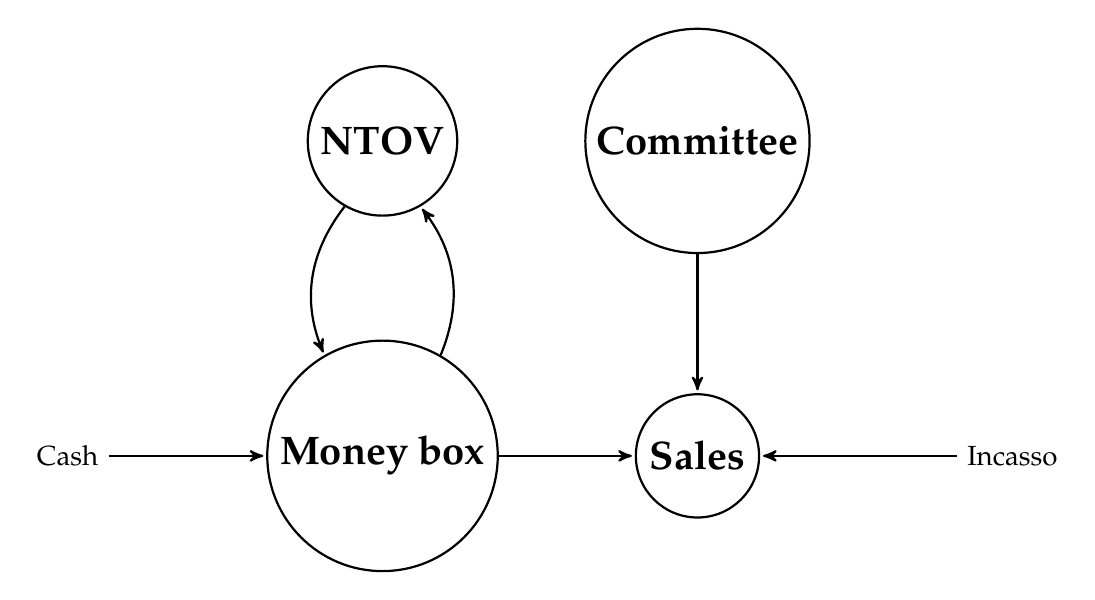
\begin{tikzpicture}[->,>=stealth',shorten >=1pt,auto,node distance=4cm,
	thick,main node/.style={circle,draw,font=\Large\bfseries}]
	
	\node[main node] (c) [midway]{NTOV};	
	\node[main node] (b) [below of=c]{Money box};
	\node[] (a) [left of=b]{Cash};
	\node[main node] (d) [right of=c]{Committee};
	\node[main node] (e) [right of=b]{Sales};
	\node[] (f) [right of=e]{Incasso};
	
	\path
	(a) edge node {} (b)
	(b) edge node {} (e)
	(d) edge node {} (e)
	(b) edge[bend right] node {} (c)
	(c) edge[bend right] node {} (b)
	(f) edge node {} (e);
	\end{tikzpicture}
	\caption{Flow chart for Drinks}
\end{figure}
\begin{figure}
	\centering
	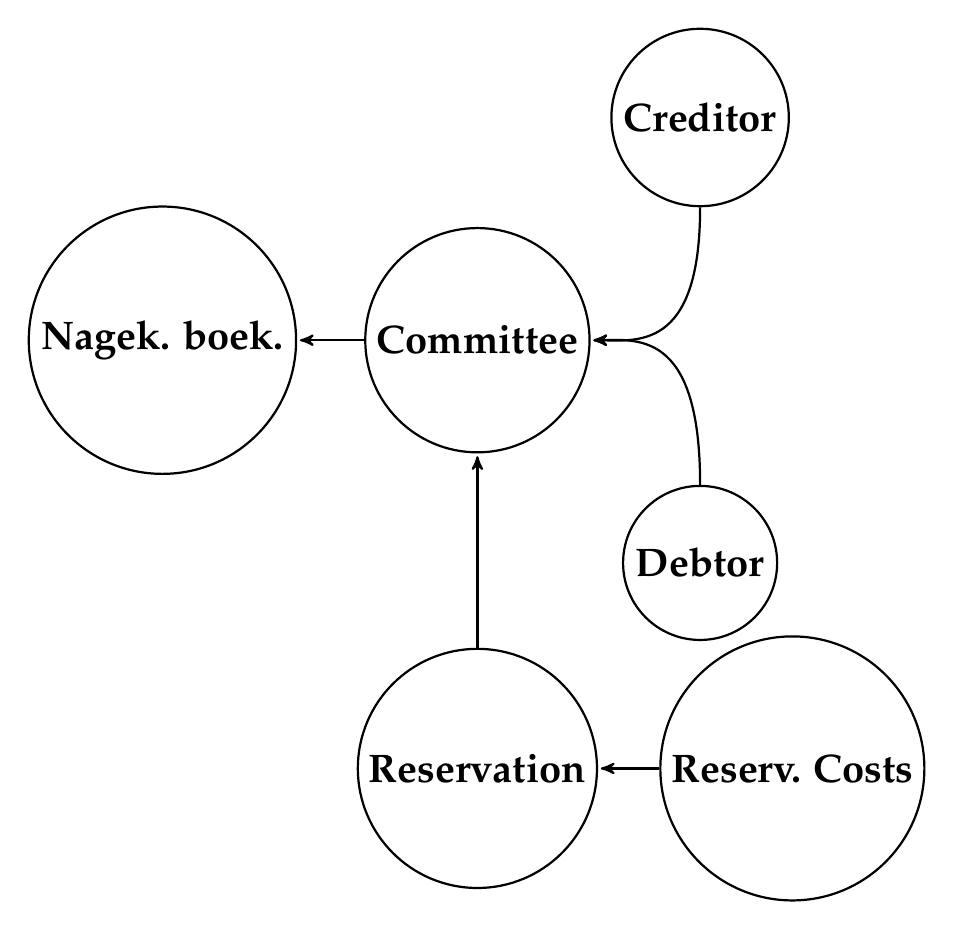
\begin{tikzpicture}[->,>=stealth',shorten >=1pt,auto,node distance=4cm,
	thick,main node/.style={circle,draw,font=\Large\bfseries}]
	
	\node[main node] (a) [midway]{Committee};
	\node[main node] (d) [midway, below of=a] {Reservation};
	\node[main node] (b) [below right of=a, align=right] {Debtor};
	\node[main node] (c) [above right of=a, align=right] {Creditor};
	\node[main node] (e) [right of=d] {Reserv. Costs};
	\node[main node] (f) [left of=a] {Nagek. boek.};
	
	\path
	(a) edge node {} (f)
	(d) edge node {} (a)
	(e) edge node {} (d);
	\draw [->] (c) .. controls +(down:3cm) and +(right:2cm) .. node[below,sloped] {} (a);
	\draw [->] (b) .. controls +(up:3cm) and +(right:2cm) .. node[above,sloped] {} (a);
	\end{tikzpicture}
	\caption{Flow chart for special committees}
\end{figure}

\mychapter{3}{Appendix}

\section{Terminology}
\subsection{Boekhouding}
typen boekhouding
welke boekhouding wij
waarom dit
\subsection{Invoice}
Whenever someone buys something from someone the way to represent that on paper is an invoice. There are a number of different invoices. The following types exist:
\begin{itemize}
\item debtor invoices
\item creditor invoices
\item simplified invoices
\item correction invoices
\end{itemize}

\subsubsection{debtor and creditor invoices}
The debtor and creditor invoices are nearly the same, the difference is that you get paid by respectively need to pay someone.

The Dutch law requires the following to be present on every debtor and creditor invoice
\begin{itemize}
	\item Name and address of the supplier
	\item Name and address of the receiver
	\item Invoice number
	\item Invoice date
	\item Date on or period in which the goods/services were supplied
	\item Quantity and type of the goods supplied
	\item Nature and type of the services supplied
	\item In case of advance payment the date of the payment
	\item VAT identification number of the supplier
	\item Price per unit excl. VAT
	\item Any price reductions not included in the price
	\item VAT tariff
	\item Total cost excl. VAT
	\item Total VAT
\end{itemize}
As some associations and companies like Abacus do not have to file a tax return, the fields VAT rules are not always applicable. In case of a debtor invoice all fields with a VAT can be omitted.

\subsubsection{Simplified invoices}\label{subsec:simplified_invoice}
The simplified invoice is either a debtor or a creditor invoice which does not go above \euro100,00 or which is a correction on a previously send invoice.
This type of invoice has less strict demands by the Dutch law. Is has to meet the following requirements:
\begin{itemize}
	\item Reference to the original invoice
	\item Name and address of the supplier
	\item Goods and services supplied 
	\item invoice date
	\item invoice amount
	\item VAT
\end{itemize}
 
\subsubsection{Other requirements by law}
All invoices are subject to additional rules. The rules discussed in the next parts are following
\begin{itemize}
	\item invoice period
	\item payment period
	\item Overdue payment
	\item invoice discount
\end{itemize}

The invoice period is the period wherein the invoice has to be sent. By Dutch law a invoice has to be sent utterly the 15th of the first month after the last goods/services have been delivered. In case the invoice is derived from a contract, the contract may overwrite this regulation. If the invoice is send late, it is invalid.

The payment period is the period in which the receiver has to pay the invoice. Once this payment period has gone by the law states that the supplier can apply a fee depending on whether the receiver is a company or consumer. This fee will be determined every semester, therefore the current fee is omitted. You can find the current fee online.

When a invoice has not been paid for too long it can get overdue. An overdue invoice does not have to be paid anymore. An invoice will get overdue after a certain while has passed since the end of the payment period. This while is dependent on what the invoice was for. Table \ref{tabl:Overdue} shows which periods are for which invoices.
\begin{table}[h]
	\centering
	\label{tab:Overdue}
	\begin{tabular}{l|l}
		Type        & Period   \\\hline \hline
		Consumerbuy & 2 years  \\\hline
		Invoice     & 5 years  \\\hline
		Default     & 20 years   	
	\end{tabular}
	\caption{Table with overdue periods}
\end{table}

Sometimes an incentive to pay an invoice early is given. This is given by a discount date with a discount amount on the invoice. Once the discount date expires the discount does no longer apply to the invoice. The height of the discount is completely up to the supplier, but the discount duration cannot be longer than the payment period.   

\subsection{Proposal} %offerte
requirements for a proposal
\begin{itemize}
	\item 
	\item 
	\item 
	\item 
	\item 
	\item 
	\item 
	\item 
\end{itemize}
Vrijblijvend
kosten alleen bij voorafgaan gemeld

\subsection{Declaration}
It is not uncommon that someone has to spent money for the association. Because it is simply unmanageable to pay yourselves all of the time, people are able to pay in advance for the association. To ensure that everyone that paid something in advance gets their money back, a document called a declaration has been made. This one can be found in the template folder on the board drive. The declaration provides the person that paid in advance to specify for which committee, when and what he or she paid in advance. To ensure that a declaration is valid he or she must fill in the following things:
\begin{itemize}
\item Post
\item Amount paid in advance
\item When the declarations is done
\item Who did the declaration
\item IBAN to deposit the amount to
\item Signature
\item Specification of what has been paid in advance
\item Receipt, bill or invoice
\end{itemize}
Note that PIN receipts are no valid receipts and that the receipt, bill or invoice should be stapled to the appointed location. When any of the things mentioned above is missing or erroneous the declaration is invalid, but may still be approved by you, if you have proper reasons to. The auditing committee will ask you for it on your next meeting.  
   
\subsection{Debtor}
Debtor is the term given for every entity owes a debt to another entity. With other words every person or company that needs to pay another person or company, e.g. ASML owing Abacus money for sponsorship or Michel Ten Bulte owing Abacus money for eating a "Speculaas Torondo". 
\subsection{Creditor}
Creditor is the term given for the entity owing money from another entity. With other words every person or company that needs to be paid, e.g. Abacus needs to pay Stichting Borrelbeheer Zilverling money for drinks or Abacus owing the Makro money for buying food and drinks. 
\subsection{Inventory/Stock}
All goods and materials the entity has that are deemed to have a some value at the point of measurement. In this should be noted that stock is meant for sale and are part of the current assets and inventory is meant be used within the company and not sold. E.g. for Abacus computers are inventory and coffee is considered stock. 
\subsection{Assets}
An asset is an economic resource. This can be everything with is deemed to have a monetary value. 
\subsubsection{Current assets}
Current assets contains everything that is reasonably to be expected to be sold, consumed or used during a single fiscal year and all money.   
\subsubsection{Fixed assets}
Fixed assets, also sometimes called long-term assets, contain everything that is not expected to be sold, consumed or used during a single year. 
\subsection{Cash}
Cash contains all money the entity has, whether it is on a bank account, in a safe or not in either. Bank accounts are also part of the cash since banks should have to give an entity all the money that is on the bank account on demand. 
\subsection{Equity capital}
Equity capital is the difference between the total of the assets and the total of the liabilities.
\subsection{Provisions}
A provision is a amount of money set aside for invoice for a past event for which the amount can be reliably estimated.
\subsection{Liquidity}
Liquidity is a measure for how well a company is able to pay its current liabilities. Usually this is done by comparing the value of everything the company has that is either money or easily changed to money to the current liabilities. Different ratio are possible, yet all share the common fact that high is good and low is bad.
\subsection{Account}
An account is a set with a name in which journal entries can be added, e.g galacommissie or crediteuren.
\section{Ledger}
A ledger is a collection of accounts or other ledgers with a name, e.g. Debiteuren '15--'16. Below here several ledgers are explained by the accounts they contain. In these explanations self-explanatory accounts are omitted.
\subsection{Room}
The Room ledger includes everything directly related to the room or the inventory, but not the stock. Since letters are written or printed in the room and calls are made from the room, these accounts are also included in the ledger. 
\subsection{Board}
The Board ledger includes everything directly related to the board, the General Member Assembly and the Honorary Members. 
\subsubsection{Clothing}
This account signifies the share that Abacus to their board members to get a proper suit. This share is a set amount for each year and the total on this account is determined by said amount and the number of board members. It is common that only the student board members receive a share.
\subsubsection{Traveling expenses and traveling expenses external affairs}
Every board travels and the association pays for that. The amounts for the Officer External Affairs is only significant enough to be separate from the general traveling expenses. 
\subsubsection{Representation}
This is an account used for giving flowers and getting utilities for the "Kandi-rondjes".
\subsubsection{Outing}
Every board receives the right to go on an outing twice as a means of bonding and as a way to give thanks. This amount is the same every year and halve of the amount is for the previous board and halve is for the current board. 
\subsubsection{Incidental}
This account contains incidental expenses associated with the board like the costs for large abaci and steam cleaning suits. 
\subsection{Association}
This ledger contains accounts that are associated with the association, yet are not suitable for other ledgers. 
\begin{itemize}
	\item Insurance $\rightarrow$ Costs for all insurances including the board liability insurance
	\item Licences $\rightarrow$ Costs for operating Multiverse
	\item Overleg Studievereningen $\rightarrow$ Membership fee for the OS
\end{itemize}
\subsection{Financial policy}
This ledger contains all accounts related to the bank, membership fees, remains of last year and losses of cash or stock.
\subsubsection{[Voorraadvershil en kasverschil]}
All financial actions should be recorded, yet sometimes an error is made during the recordings. These errors can lead to a different stock or amount of cash than expected by the recorded transactions. If the error cannot or is not found and corrected, the difference between the expected amount and current amount is placed on this account, such that the stock and cash meets their expected amounts. 
\subsubsection{[Nagekomen boekingen]}
In most years it happens that something happens that should have fallen in the fiscal year before the current one, yet the previous fiscal year has already closed, so these transactions are placed on this account. This can also be the remainder of a provision or reserve after the invoices have been paid.  
\subsection{Sales}
Sales contain all the products sold aside from coffee, thee and chocolate milk or products sold during drinks or activities. All consumables are put under [versnaperingen] and all stock with a small enough number or that has a limited edition.     
\subsection{Activities}
This ledger contains all accounts related to committees or lectures or excursions.
\subsection{Association printed matter}
This is the post for the \textit{Ideaal!} and the almanac committee. 
\subsubsection{Posts for printed matter}
Abacus has also other printed matter, but those belong to other posts. The list belong links the printed matter to the proper post:
\begin{itemize}
\item Paper and ink in the Abacus room 		$\rightarrow$ Kantoorbehoeften
\item Paper for the General Member Assemble $\rightarrow$ ALV kosten
\item Mini-almanac $\rightarrow$ Eerstejaarscommissie
\item Poster or promotion material $\rightarrow$ Committee that does the promoting
\end{itemize}
The reason for this is that by setting printed matter to the committee a better estimate of the costs can be made for printing. This is a result of that it is easier to see what the printing costs are when it is on the same budget as where the printing is for compared to just having a number that is a result of adding all printing matter together.
\subsubsection{Almanac committee}
The almanac committee is a committee that sole purpose is to produce a almanac. This is a printed product, so it is natural for it to be here.

\subsection{Drink}
\subsubsection{Abacus Drink}
\begin{itemize}
\item (A)bac(ch)us drink
\item Ab-Actie drink
\item Remaining drinks
\end{itemize}
\subsubsection{External Drink}
\begin{itemize}
\item Graduation drink
\item Faculty drink
\item Association drink
\item Non-uni drink
\end{itemize}
\subsection{Active Member}
\subsubsection{Active Member Weekend}
Once a year the board shall organize a weekend for which all the active members and a part of the past boards will be invited. The weekend is depicted with a drink on the Friday, the early risers drink, a game leading everyone to the campsite and a weekend full of games organized by the board. 

As it is a whole weekend for active members the expanses are not going to be low, so a budget has te be made for this. Make sure you account for the following:
\begin{itemize}
	\item A campsite
	\item A truck for moving luggage
	\item Breakfast for the early risers drink and for both days on the campsite
	\item Diner for the Saturday
	\item Plenty of drinks and snacks
	\item Games and prizes
	\item Travel expenses 
\end{itemize}
Note the travel expenses. As it is a weekend at a remote location for the active members and old boards, everyone should have the opportunity to get to the campsite without large expanses. Therefor it is customary to refund the travel expanses.
 
\subsubsection{Active Member Thank Drink}
Once in the year the board will organize a drink for all active members to say thanks to them. It is customary to give a gift to the active members. Usually the number of gifts exceeds the number of active members that collect there gift. Once everyone came to collect there gift and the number of gifts is still reasonably high the gifts can be placed in storage, so that they can be sold the year after. 
\subsection{Sponsoring}
\subsection{Faculty}
This is the post for money received by the faculty. Once in the year the amount will be set. The amount you will receive depends on the number of legible students and the amount per legible student. As this value is set every year, it is not unlikely you are going to receive a different amount than you put/will put in your budget.
\subsection{New initiatives}
In your year as treasurer it is likely you are going to want to buy something new. If the new thing doesn't have a right fit in one of the other existing posts, then this is the post you want to place it on.
\subsection{Contingencies}
Some things you simple are not able to predict, but do cost Abacus some money. The incidents that cause these costs are put to the contingencies post. With Abacus those incidents rarely happen, so it is common practice to not reserve any money for contingencies. Examples of what might be such an incident are costs for repairing the dish washer or a broken window.
\section{Direct Debit}
\subsection{First and recurrent direct debits}
\subsection{Place a direct debit order}
\section{Website}
\subsection{Track and archive direct withdrawal state}
\subsection{Create a direct withdrawal order}
\subsection{Send mail for direct withdrawal}
\section{Multivers}
Multivers is the accounting program you will be using. It serves as the digital collection of all your financial actions and transactions. The use of such a program greatly enhances the overview you have and greatly reduces the amount of errors going unnoticed.
\section{Troubleshoot}
\subsection{Send an erroneous invoice}
In case you noticed that you have sent and erroneous invoice, you should sent a correction invoice. A correction invoice is can be made in either of two ways which are both valid. 
The first way to make a correction invoice is by making a completely new invoice with the new amount, but also add the old amounts as negatives.
The second way is to make a new invoice with only amounts that represent the difference between what should have been paid and what has been paid. 
Both ways require that you reference to the erroneous invoice. Please note that the newer invoice has to have a sequentially higher number in your administration. Further note that in case you make a correction invoice not all information that is required on a ordinary invoice has to be present as the correction invoice is a subset of the simplified invoices, see for more information \ref{subsec:simplified_invoice}.

\subsection{Overdue payment}
\subsection{Refusal to pay}
\subsection{Blocked direct withdrawal}
\section{Best practices}
\subsection{Naming conventions}
\subsection{Ordering multivers}
\subsection{Regular actions}
\subsection{Accepting stuff}
\section{Auditing committee}
Quick Ratio
Liquidity Ratio
Current Ratio
\subsection{Kascosheet}
\subsection{Documents to deliver on auditing session}
\subsection{Documents that need auditing}
\section{Archive}
\begin{itemize}
	\item What to archive
	\item What to keep close
\end{itemize}
immovable property 10 years
rest 7 years
\section{Glossary}
\end{document}